\section{Evaluation Results}
\label{sec:snic:results}

We implemented \snic\ on the HiTech Global HTG-9200 board~\cite{htg9200}. 
Each board has nine 100\Gbps\ ports, 10\GB\ on-board memory, and a Xilinx VU9P chip with 2,586K LUTs and 43\MB\ BRAM.
We implemented most of \snic's data path in SpinalHDL~\cite{SpinalHDL} and \snic's control path in C (running in a MicroBlaze SoftCore~\cite{microblaze-xilinx} on the FPGA).
Most data path modules run at 250 MHz.
In total, \snic\ consists of 8.5K SLOC (excluding any \nt\ code).
The core \snic\ modules consume less than 5\% resources of the Xilinx VU9P chip, leaving most of it for \nt{}s (see Appendix for full report).
To put it in perspective, the Go-back-N reliable transport we implement consumes 1.3\% LUTs and 0.4\% BRAM.

\bolditpara{Environment.}~~ 
We perform both cycle-accurate simulation (with Verilator~\cite{verilator-site}) and real end-to-end deployment.
Our deployment testbed is a rack with a 32-port 100\Gbps\ Ethernet switch, two HTG-9200 boards acting as two \snic{}s, eight Dell PowerEdge
R740 servers, each equipped with a Xeon Gold 5128 CPU and an NVidia 100\Gbps\ ConnectX-4 NIC, and two Xilinx 10\Gbps\ ZCU106 boards running as Clio~\cite{clio-arxiv} disaggregated memory devices.
Each \snic\ uses one port to connect to the ToR switch and one port to connect to the other \snic.
Depending on different evaluation settings, an \snic{}'s downlinks connect to two servers or two Clio devices.

{
\begin{figure*}[th]
\begin{center}
\centerline{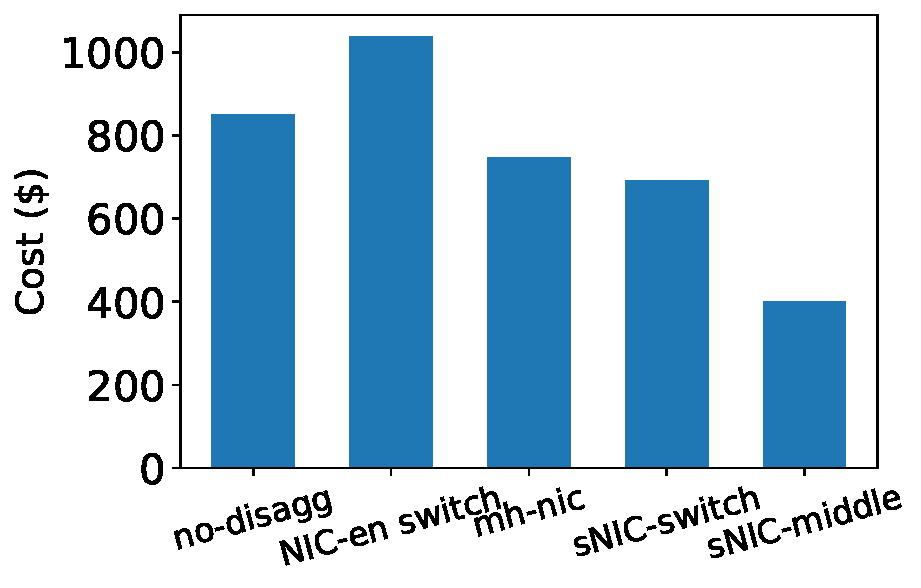
\includegraphics[width=0.5\textwidth]{snic/Figures/fig-single-rack-capex-perDevCost.pdf}}
\mycaption{fig-rack-capex}{Per-Endpoint CapEx.}
{
A rack's network cost divided by endpoint count. 
}
\end{center}
\end{figure*}
}
{
\begin{figure*}[h]
\begin{center}
\centerline{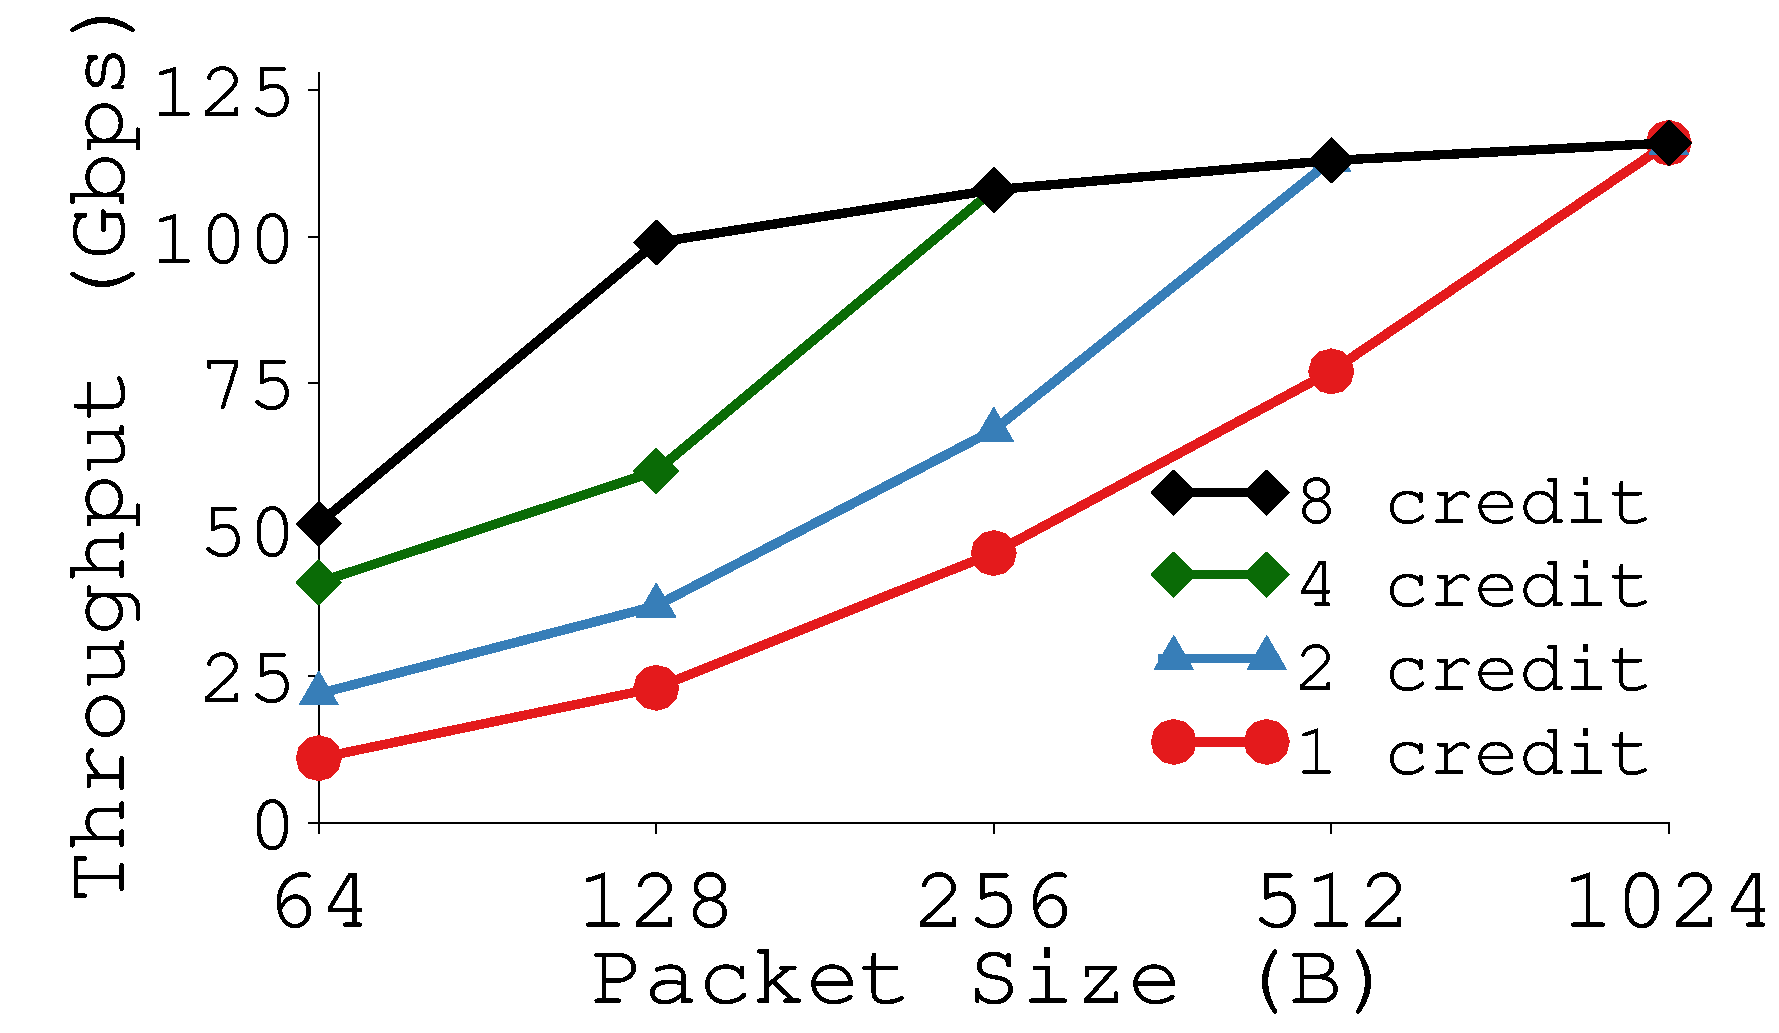
\includegraphics[width=0.5\textwidth]{snic/Figures/g_plot_credit.pdf}}
\mycaption{fig-credit}{Throughput with different credits.}
{
}
\end{center}
\end{figure*}
}
{
\begin{figure*}[h]
\begin{center}
\centerline{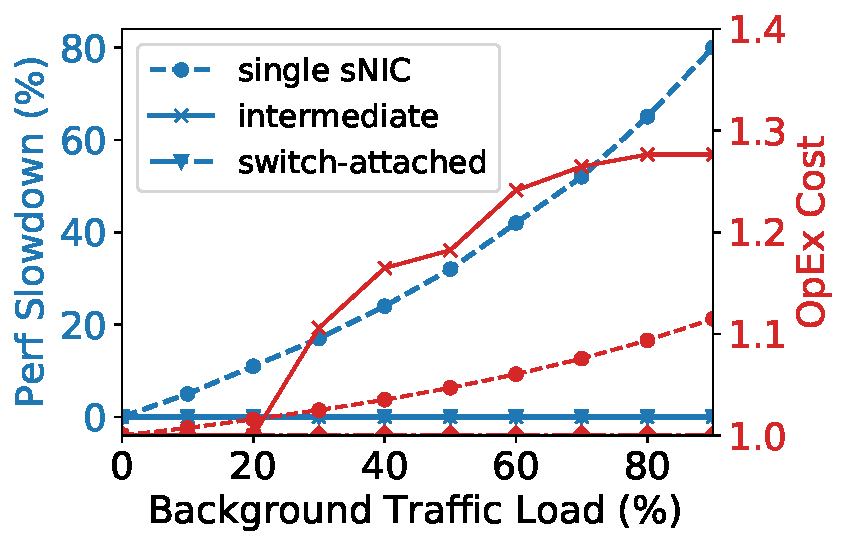
\includegraphics[width=0.5\textwidth]{snic/Figures/fig-dist-nic-load-increase.pdf}}
\mycaption{fig-sim-dist-nic}{Distributed \snic{}.}
{
}
\end{center}
\end{figure*}
}
{
\begin{figure*}[h]
\begin{center}
\centerline{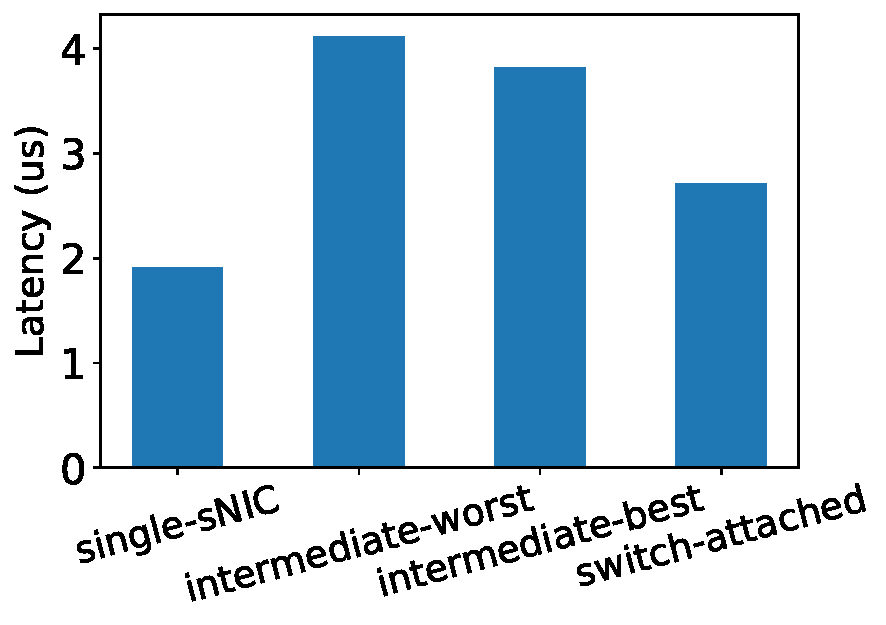
\includegraphics[width=0.5\textwidth]{snic/Figures/fig-dist-nic-latency.pdf}}
\mycaption{fig-topology-cmp}{Topology Comparison.}
{
}
\end{center}
\end{figure*}
}

\subsection{Overall Performance and Costs}
\label{sec:snic:eval-overview}

\bolditpara{CapEx cost saving.}~~
We compare the CapEx cost of \snic's two architectures with no network disaggregation, traditional multi-host NIC, and traditional NIC-enhanced switches.
All calculations are based on a single rack and include 1) endpoint NICs, 2) cables between endpoints, \snic{}s, and the ToR switch, 3) the ToR switch, and 4) cost of \snic{}s or multi-host NICs.
We use market price when calculating the price of regular endpoint NICs and cables.
With \snic, the endpoint NICs can be shrunken down to physical and link layers (based on our prototype estimation, it is roughly 20\% of the original NIC cost of \$500), and the cables connecting endpoints and \snic{}s in the middle-layer-pool architecture can be shortened (roughly 60\% of the original cable cost of \$100~\cite{RAIL-NSDI}).
We estimate the ToR-switch cost based on the number of ports it needs to support and a constant per-port cost of \$250~\cite{fs-64port-switch}.

To estimate the cost of an \snic, we separate the non-\nt\ parts and the \nt\ regions. The former has a constant hardware cost, while the latter can be provisioned to the peak of aggregated traffic and \nt\ usages, both of which are workload dependent. We use the peak-of-sum to sum-of-peak ratios obtained from the Facebook traces (\S\ref{sec:snic:benefits}). Today's multi-host NIC and NIC-enhanced switches do not consolidate traffic, and we assume that they will be provisioned for the sum-of-peak. See Appendix for detailed calculation. 

Figure~\ref{fig-rack-capex} plots the per-endpoint dollar CapEx cost. Overall, \snic\ achieves \textbf{52\% and 18\% CapEx savings} for the middle-layer and switch-attached pool architecture compared to no disaggregation.
Multi-host NIC and NIC-enhanced switches both have higher CapEx costs than \snic, because of its high provisioning without auto-scaling. The NIC-enhanced switches are even more costly than traditional racks mainly because of the added switch ports and NICs.

\bolditpara{OpEx saving and single-\snic\ performance.}~~
We compare a single \snic\ connecting four endpoints with the baseline of no disaggregation when these endpoints each run its \nt{}s on its own SmartNIC.
We generate workloads for each endpoint based on the Facebook memcached dataset distributions~\cite{Atikoglu12-SIGMETRICS}.
For the per-endpoint SmartNIC, we statically allocate the hardware resources that can cover the peak load.
Overall, we found that \snic\ achieves \textbf{56\% OpEx saving}, because \snic\ dynamically scales the right amount of hardware resources for the aggregated load.
\snic\ only adds \textbf{only 4\% performance overhead} over the optimal performance that the baseline gets with maximum allocation.

%\bolditpara{Single \snic\ throughput.}~~
We then test the throughput a real \snic\ board can achieve with a dummy \nt.
These packets go through every functional module of the \snic, including the central scheduler and the packet store. 
We change the number of initial credits and packet size to evaluate their effect on throughput, as shown in Figure~\ref{fig-credit}.
These results demonstrate that our FPGA prototype of \snic\ could reach more than 100\Gbps\ throughput. 
With higher frequency, future ASIC implementation could reach even higher throughput.
%Similar to PANIC~\cite{panic-osdi20}, we find that having more initial credits achieves higher throughput, and 8 credits are enough for 100\Gbps\ network.

Next, we evaluate the latency overhead a real \snic\ board adds.  
It takes 1.3\mus\ for a packet to go through the entire sNIC data path. % (PHY, MAC, sNIC core, MAC, and PHY). 
Most of the latency is introduced by the third-party PHY and MAC modules, which could potentially be improved with real ASIC implementation and/or a PCIe link. 
The \snic\ core only takes 196\,ns.
Our scheduler achieves a small, fixed delay of 16 cycles, or 64\,ns with the FPGA frequency. 
%The synchronization buffer has an overhead of 4 cycles, or 16\,ns.
To put things into perspective, commodity switch's latency is around 0.8 to 1\mus.  

\bolditpara{Distributed \snic{}s.}~~
To understand the effect of distributed \snic\ pool, we compare the two pool topology with a single \snic\ (no distributed support).
Figure~\ref{fig-sim-dist-nic} shows the performance and OpEx cost.
Here, we use the workload generated from the Facebook distribution as the foreground traffic and vary the load of the background traffic.
As background load increases, a single \snic\ gets more over-committed and its performance becomes worse.
With distributed \snic, we use an alternative \snic{} to handle the load, thus not impacting the foreground workload's performance. Note that the background workload's performance is not impacted either, as long as the entire \snic\ pool can handle both workloads' traffic. Furthermore, these workloads are throughput oriented, and we achieve max throughput with distributed \snic{}s.
As for OpEx, the intermediate-pool topology uses one \snic\ to redirect traffic to the other \snic.
As the passthrough traffic also consumes energy, its total OpEx increases as the total traffic increases.
The switch-attached topology does not have the redirecting overhead.
The single \snic\ also sees a higher OpEx as load increases because the workload runs longer and consumers more energy.

We then compare the two topologies of \snic\ pool. % and with no disaggregation. 
Figure~\ref{fig-topology-cmp} shows the latency comparison.
%As expected, no disaggregation achieves the best latency, as it does not need any additional network hops. 
The intermediate-pool topology where we connect the \snic{}s using a ring has a range of latency depending on whether the traffic only goes through the immediately connected \snic\ (single-\snic) or needs to be redirected to another \snic\ when the immediate \snic\ is overloaded. 
Because of the ring connection, this other \snic's distance to the immediately connected \snic\ determines the additional latency incurred (intermediate-best and worst).
In contrast, the switch-attached topology has a constant latency, even when one or multiple \snic{}s are overloaded. This is because the traffic always goes through the switch which directs it to the right \snic.

{
\begin{figure*}[th]
\begin{center}
\centerline{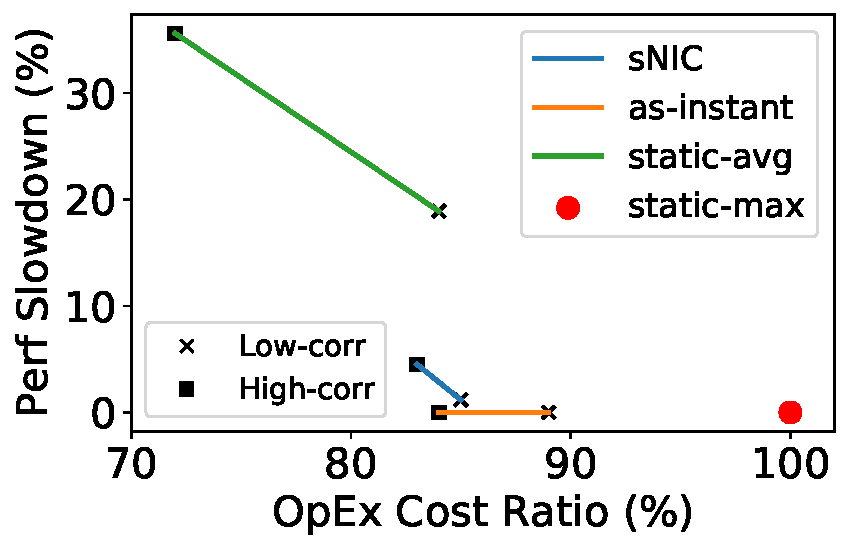
\includegraphics[width=0.5\textwidth]{snic/Figures/fig-conslid-overview-new.pdf}}
\mycaption{fig-sim-overview}{Performance and OpEx Overview.}
{
Lower is better for both axis.
}
\end{center}
\end{figure*}
}
{
\begin{figure*}[h]
\begin{center}
\centerline{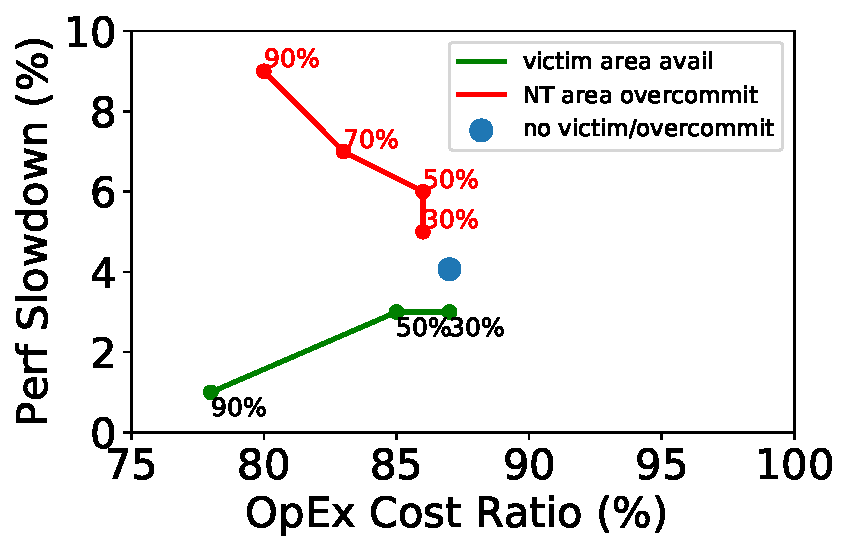
\includegraphics[width=0.5\textwidth]{snic/Figures/fig-single-snic-low-corr.pdf}}
\mycaption{fig-sim-single-snic}{Single \snic{} Sensitivity.}
{
Each lines is running a different set of experiments.
}
\end{center}
\end{figure*}
}
{
\begin{figure*}[h]
\begin{center}
\centerline{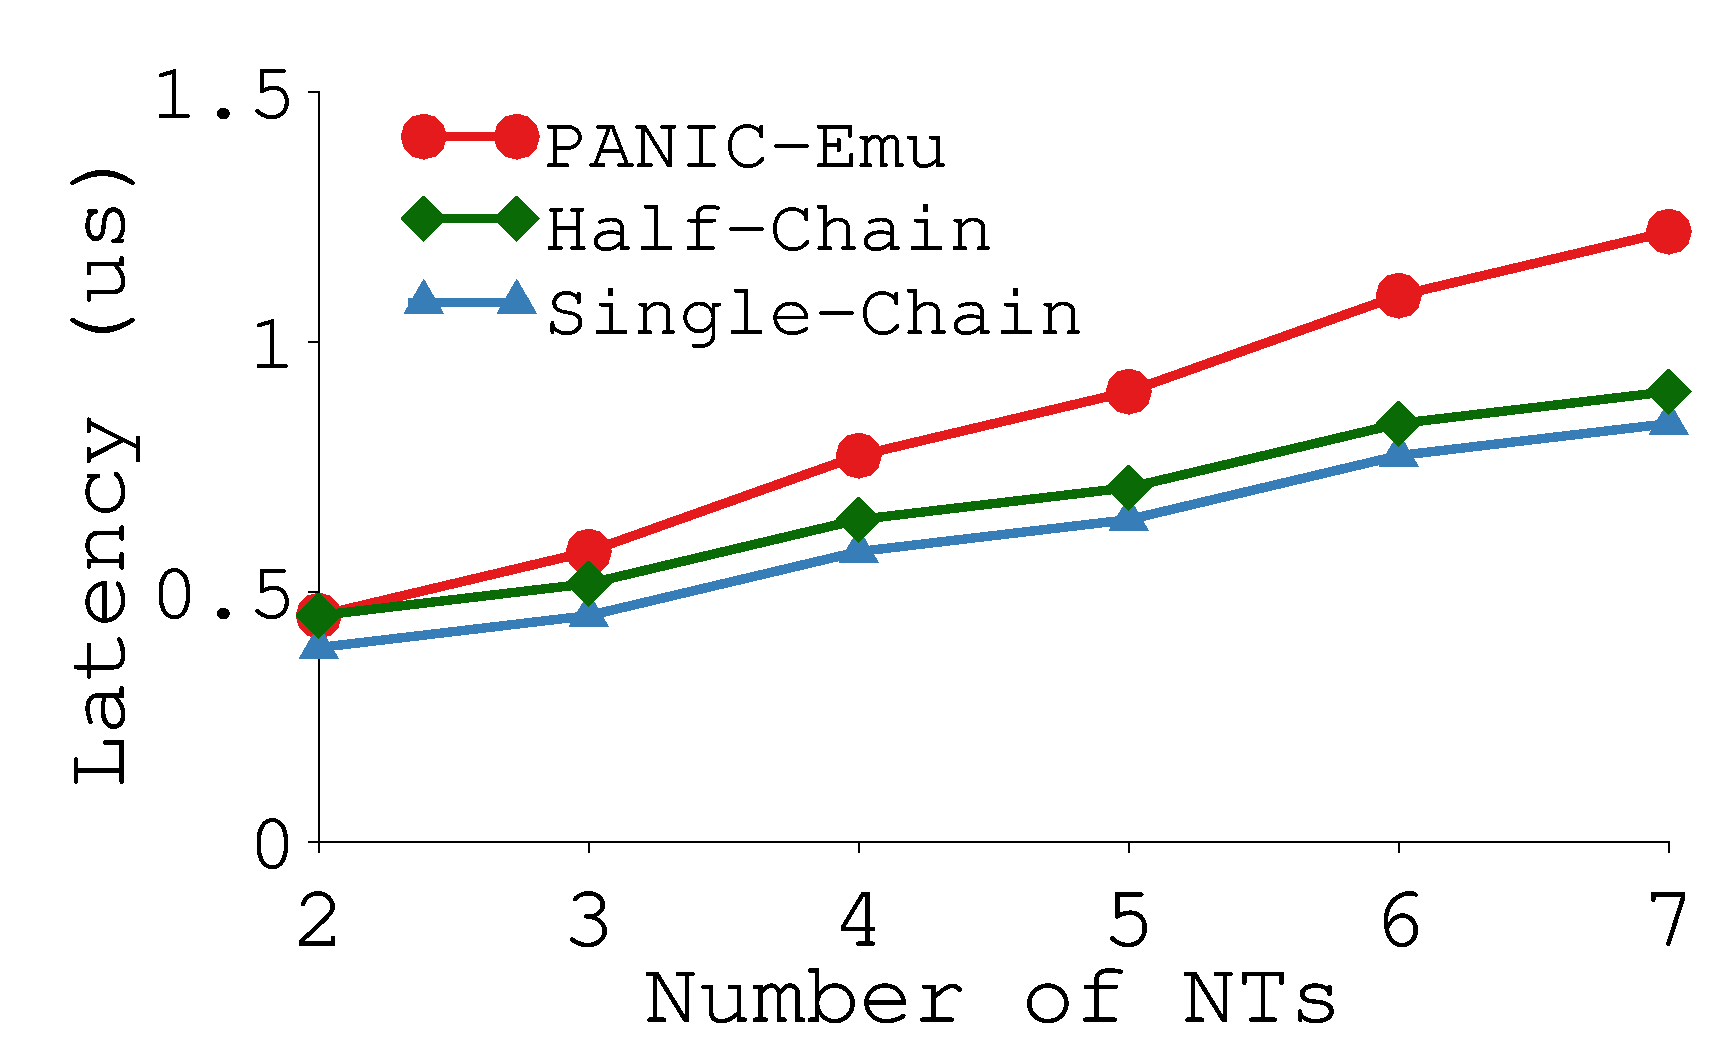
\includegraphics[width=0.5\textwidth]{snic/Figures/g_plot_nt_chain.pdf}}
\mycaption{fig-nt-chain}{\nt{} Chain.}
{
}
\end{center}
\end{figure*}
}
{
\begin{figure*}[h]
\begin{center}
\centerline{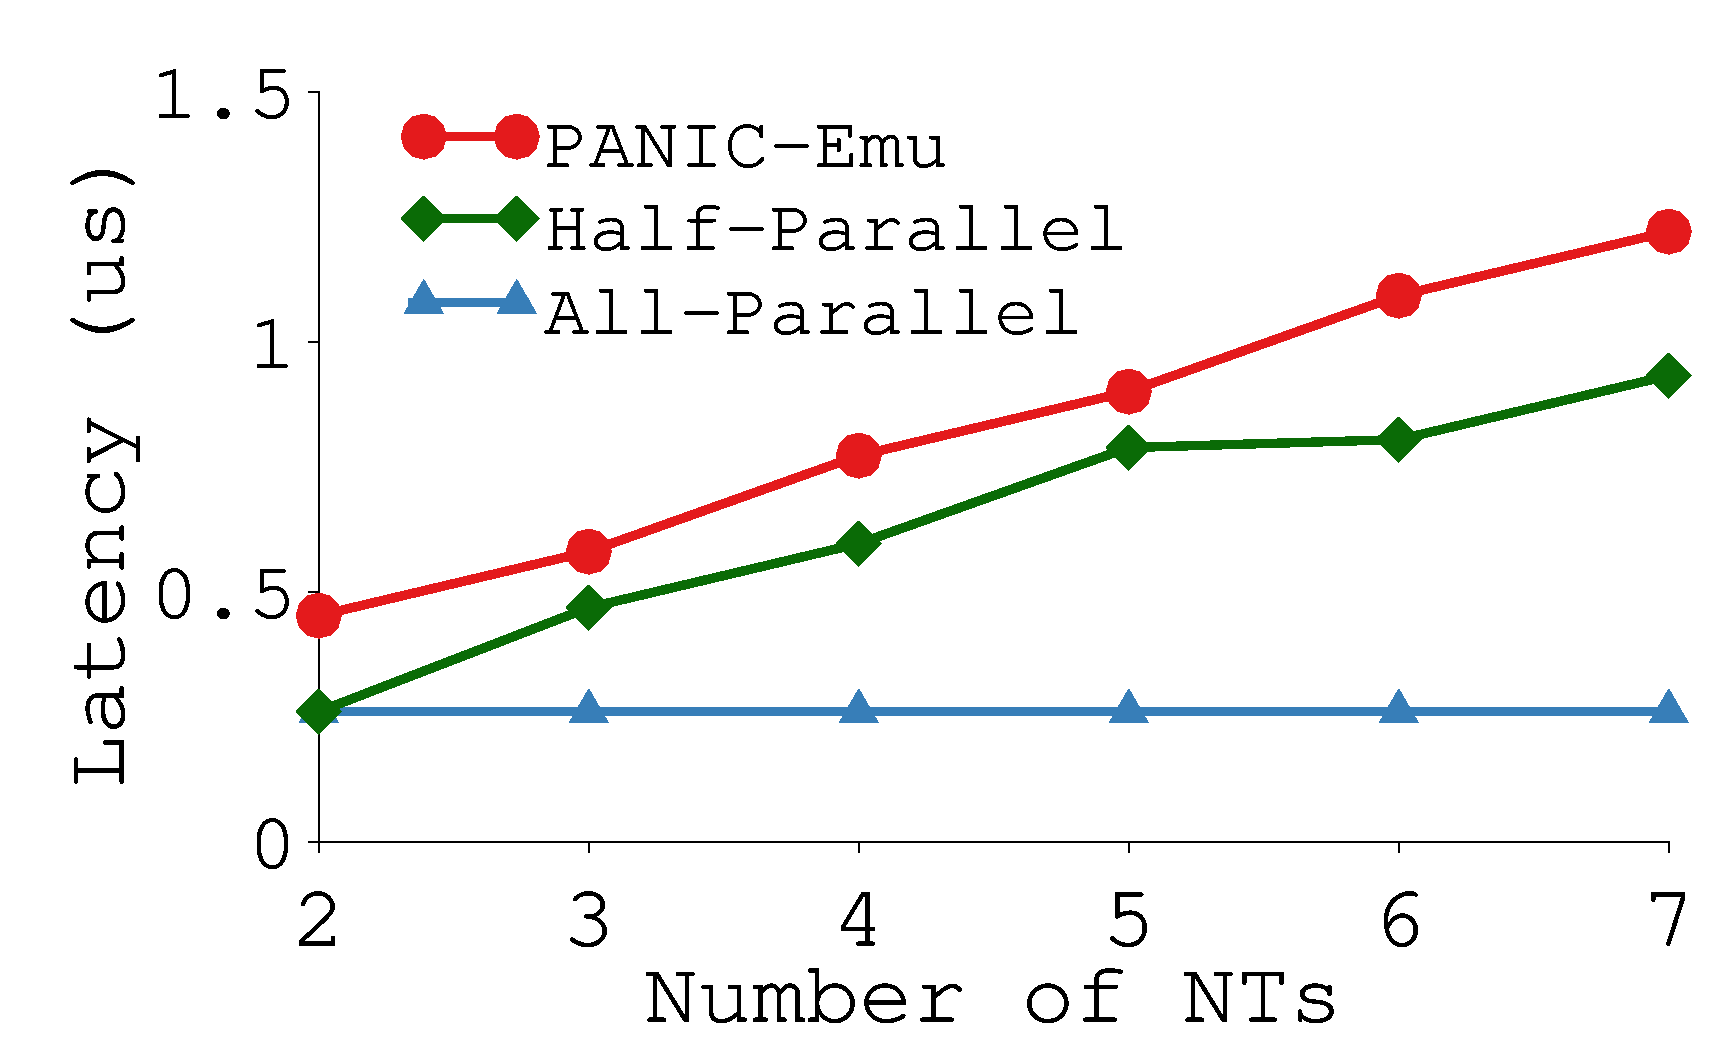
\includegraphics[width=0.5\textwidth]{snic/Figures/g_plot_nt_parallel.pdf}}
\mycaption{fig-nt-parallel}{\nt{} Parallelism.}
{
}
\end{center}
\end{figure*}
}

\subsection{Deep Dive into \snic\ Designs}
\label{sec:snic:deepdive}

We now perform a set of experiments to understand the implications of \snic's various designs in terms of performance and OpEx cost, also with the Facebook distribution.
%We calculate OpEx cost as the amount of and duration of hardware resources used. 
%For these experiments, we generate workloads also from the same Facebook distributions.

\bolditpara{Effect of auto-scaling.}~~
We compare our auto-scaled implementation of \snic\ with two types of static allocations (\ie, no load-based scaling): allocating for the highest load needs ({\em static-max}) and allocating for the average load needs ({\em static-avg}), and an unrealistic auto-scaled scheme which instantly scales the right amount of \nt\ instances as load changes and incurs zero context switching overhead ({\em as-instant}).
We generate two workloads using the Facebook distributions, one where different endpoints spike at similar time (high correlation) and one where they spike at different times (low correlation).
Figure~\ref{fig-sim-overview} shows the performance slowdown (compared to no network disaggregation) and OpEx costs (compared to static-max).

\snic\ is at the Pareto frontier compared to the two static allocation schemes. Static-max has the best performance but the worst OpEx cost, as it pays for the peak hardware resources for the entire duration. In contrast, static-avg has the worst performance but best OpEx cost, since it only allocates the resource for the average usage for the entire duration.
Compared to \snic, as-instant only achieves slightly better performance with slightly more OpEx spending, as it tightly matches resources to the load which is unrealistic.

Comparing the two workloads, the low-correlation one always has better performance and more OpEx spending than the high-correlation one (except for as-instant which always yields best performance and static-max which always yields best performance and worst OpEx).
This is because with low correlation, the aggregated traffic is more flattened out, which gives \snic\ better chance to properly handle. As a result, \snic\ scales the right amount of resources to satisfy the load's performance needs.
When correlation is high (which is unlikely from our trace analysis in \S\ref{sec:snic:benefits}), there will be fewer but more intensive spikes. When \snic\ is not fast or powerful enough to handle some of them, less resources is used but the performance goes down.

\bolditpara{Effect of victim cache.}~~
To evaluate the effect of our victim-cache design, we set the baseline to be disabling victim cache (blue dot in Figure~\ref{fig-sim-single-snic}).
We then change how often a de-scheduled \nt\ can be kept around as a victim instead of being completely deleted (shown as percentage on the green line). 
This configuration models how often an \snic's area is free to host victim \nt{}s.
As expected, the more de-scheduled \nt{}s we can keep around, the better performance we achieve, with no victim cache (baseline) having the worst performance.
The OpEx implication is less intuitive.
Here, we only count the time and amount of \nt\ regions that are actually accessed, as only those will cause the dynamic power (when idle, FPGA has a static power consumption regardless of how it is programmed).
With fewer de-scheduled \nt{}s kept around, more \nt{}s need to be re-launched (through FPGA PR) when the workload demands them. 
These re-launching overhead causes the OpEx to also go up.

\bolditpara{Effect of area over-commitment.}~~
We change the degree of area over-commitment by limiting how much hardware resources (\ie, NT regions) the workload can use compared to the ideal amount of resources needed to fully execute it.
%which is the amount of resources actually used over the total amount of hardware resources needed to execute the workload without context switching.
As Figure~\ref{fig-sim-single-snic} shows, as we increase the area over-commitment rate, we see worse performance and less resources (OpEx) used. 
Thus, our design uses distributed \snic{}s to avoid the over-commitment of a single \snic.

\bolditpara{\nt\ chaining.}~~
To evaluate the effect of \snic's \nt-chaining technique, we change the length of \nt\ sequence from 2 to 7 (as prior work found real NFs are usually less than 7 in sequence~\cite{NFP-sigcomm17}).
In comparison, we implemented PANIC's scheduling mechanism on our platform, so that everything else is the same as \snic.
We also evaluate the case where \snic\ splits the chain into two sub-chains.
Figure~\ref{fig-nt-chain} shows the total latency of running the \nt\ sequence with these schemes.
\snic\ outperforms PANIC because it avoids going through the scheduler during the sequence for single-chain and only goes through the scheduler once for half-chain.

{
\begin{figure*}[t]
\begin{center}
\centerline{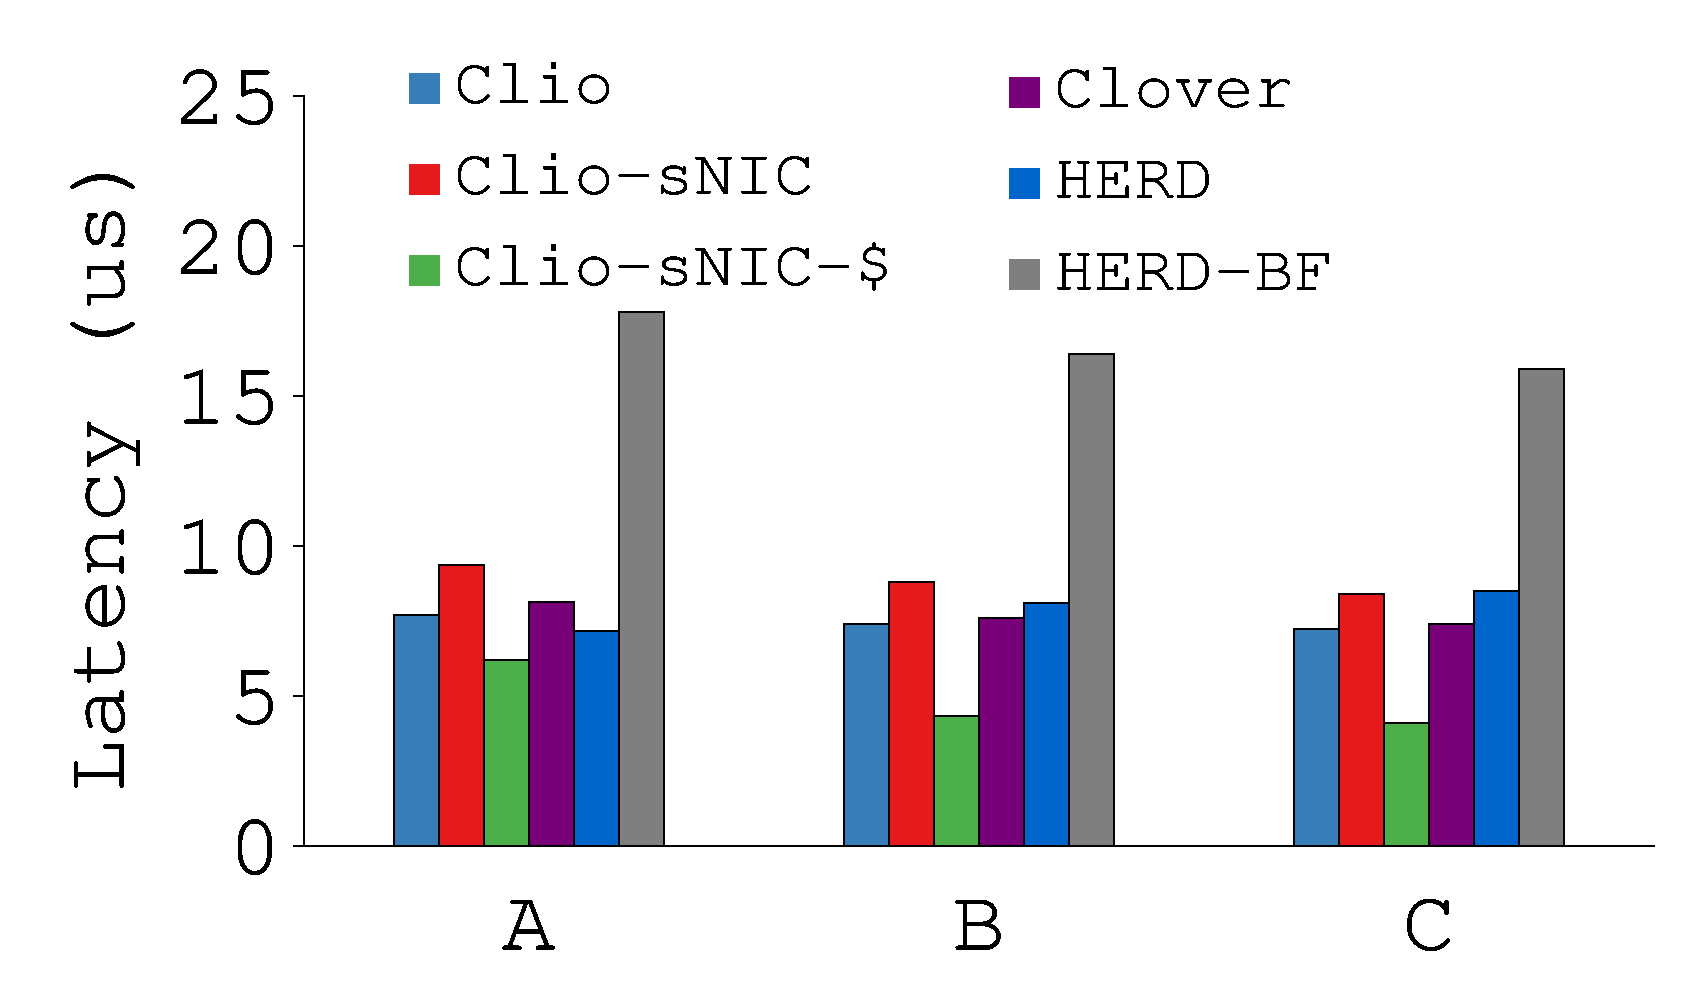
\includegraphics[width=0.5\textwidth]{snic/Figures/g_plot_ycsb.pdf}}
\mycaption{fig-snic-ycsb}{YCSB Latency.}
{
}
\end{center}
\end{figure*}
}
{
\begin{figure*}[h]
\begin{center}
\centerline{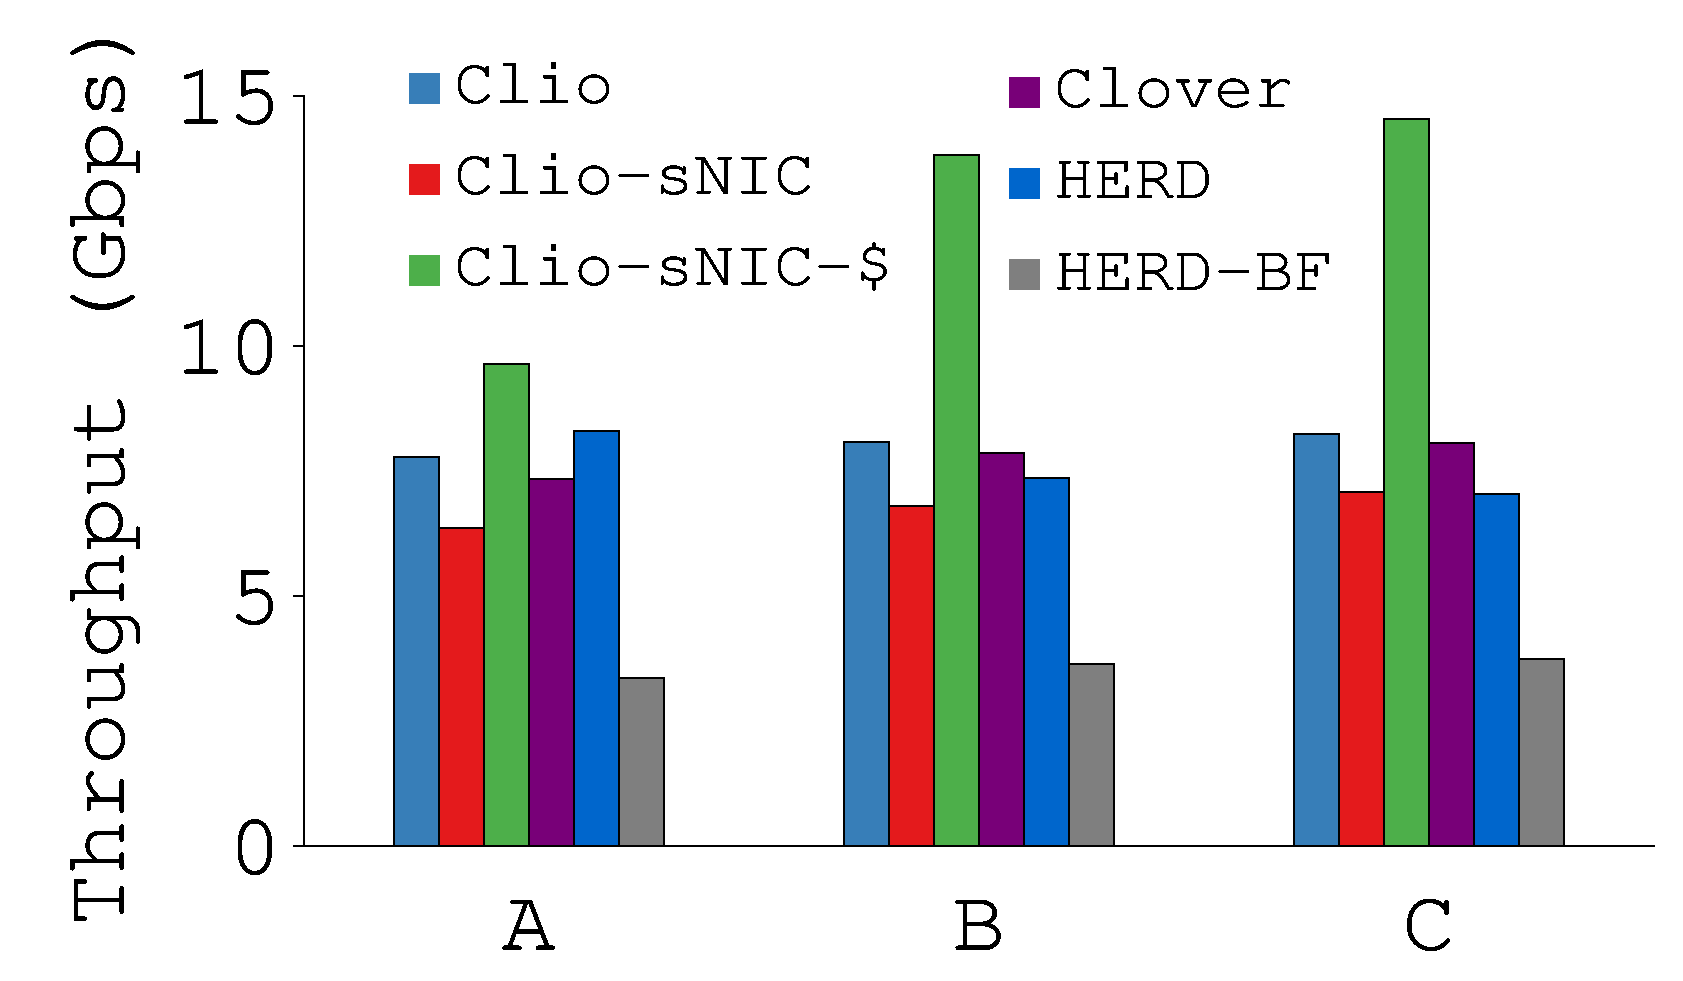
\includegraphics[width=0.5\textwidth]{snic/Figures/g_plot_ycsb_throughput.pdf}}
\mycaption{fig-snic-ycsb-tput}{YCSB Throughput.}
{
}
\end{center}
\end{figure*}
}
{
\begin{figure*}[h]
\begin{center}
\centerline{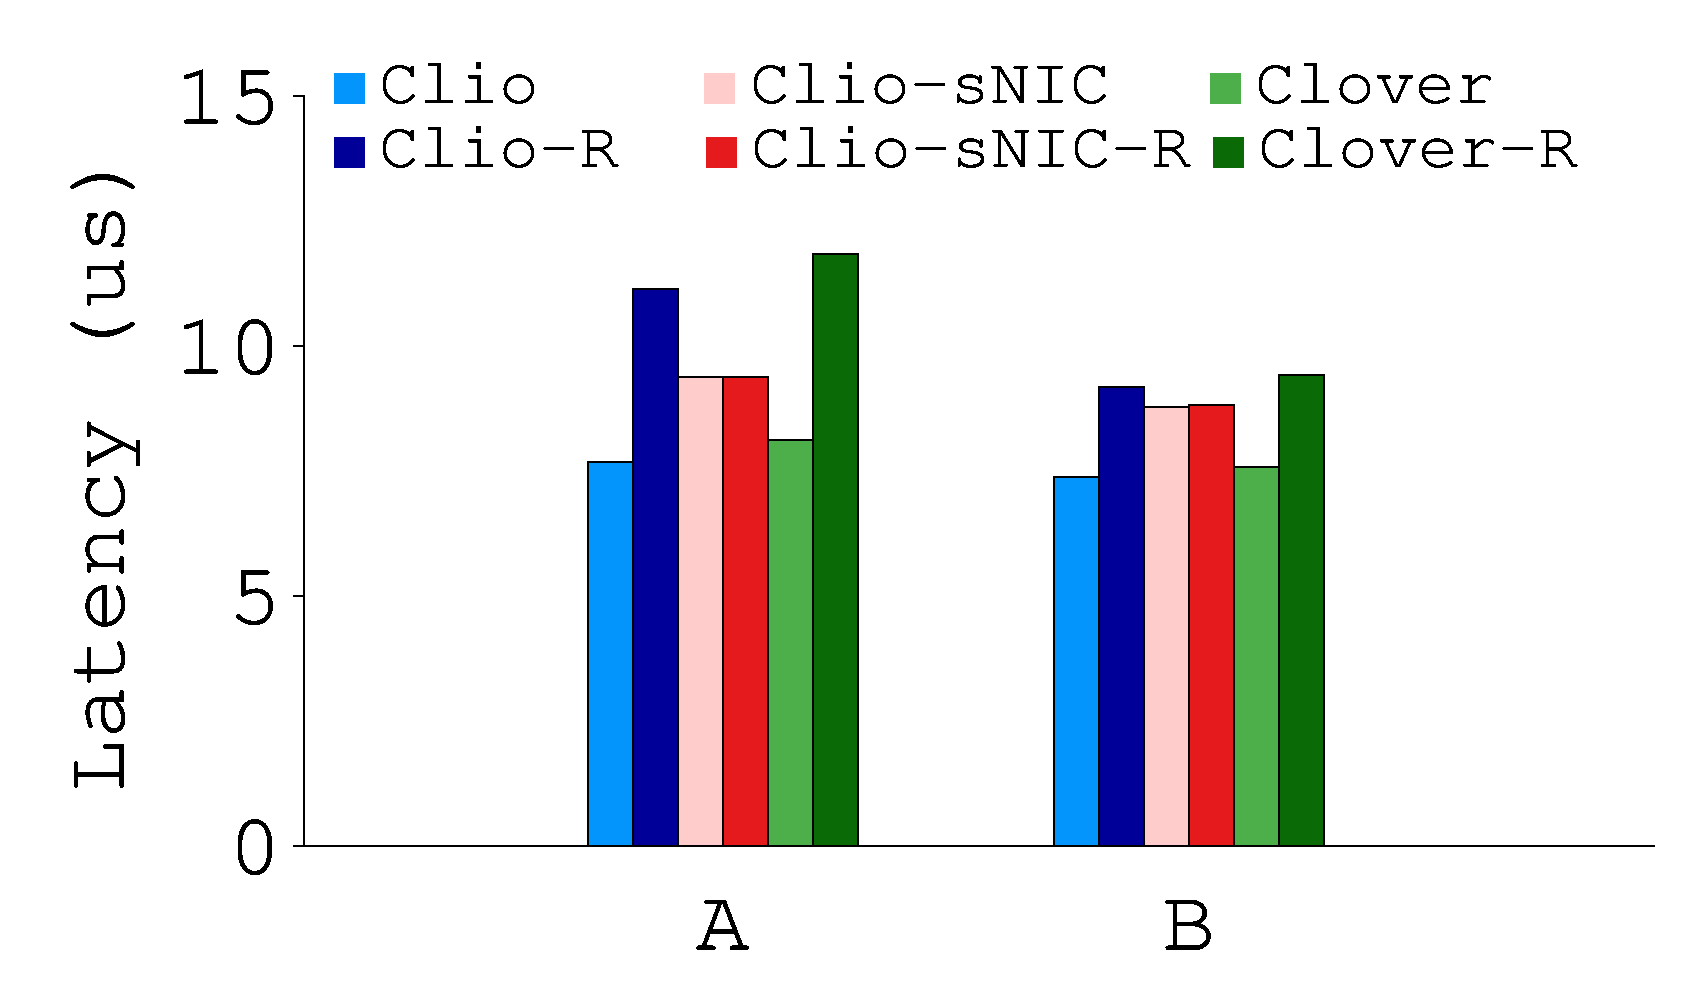
\includegraphics[width=0.5\textwidth]{snic/Figures/g_plot_ycsb_replication.pdf}}
\mycaption{fig-ycsb-replication}{Replicated YCSB.}
{
}
\end{center}
\end{figure*}
}
{
\begin{figure*}[h]
\begin{center}
\centerline{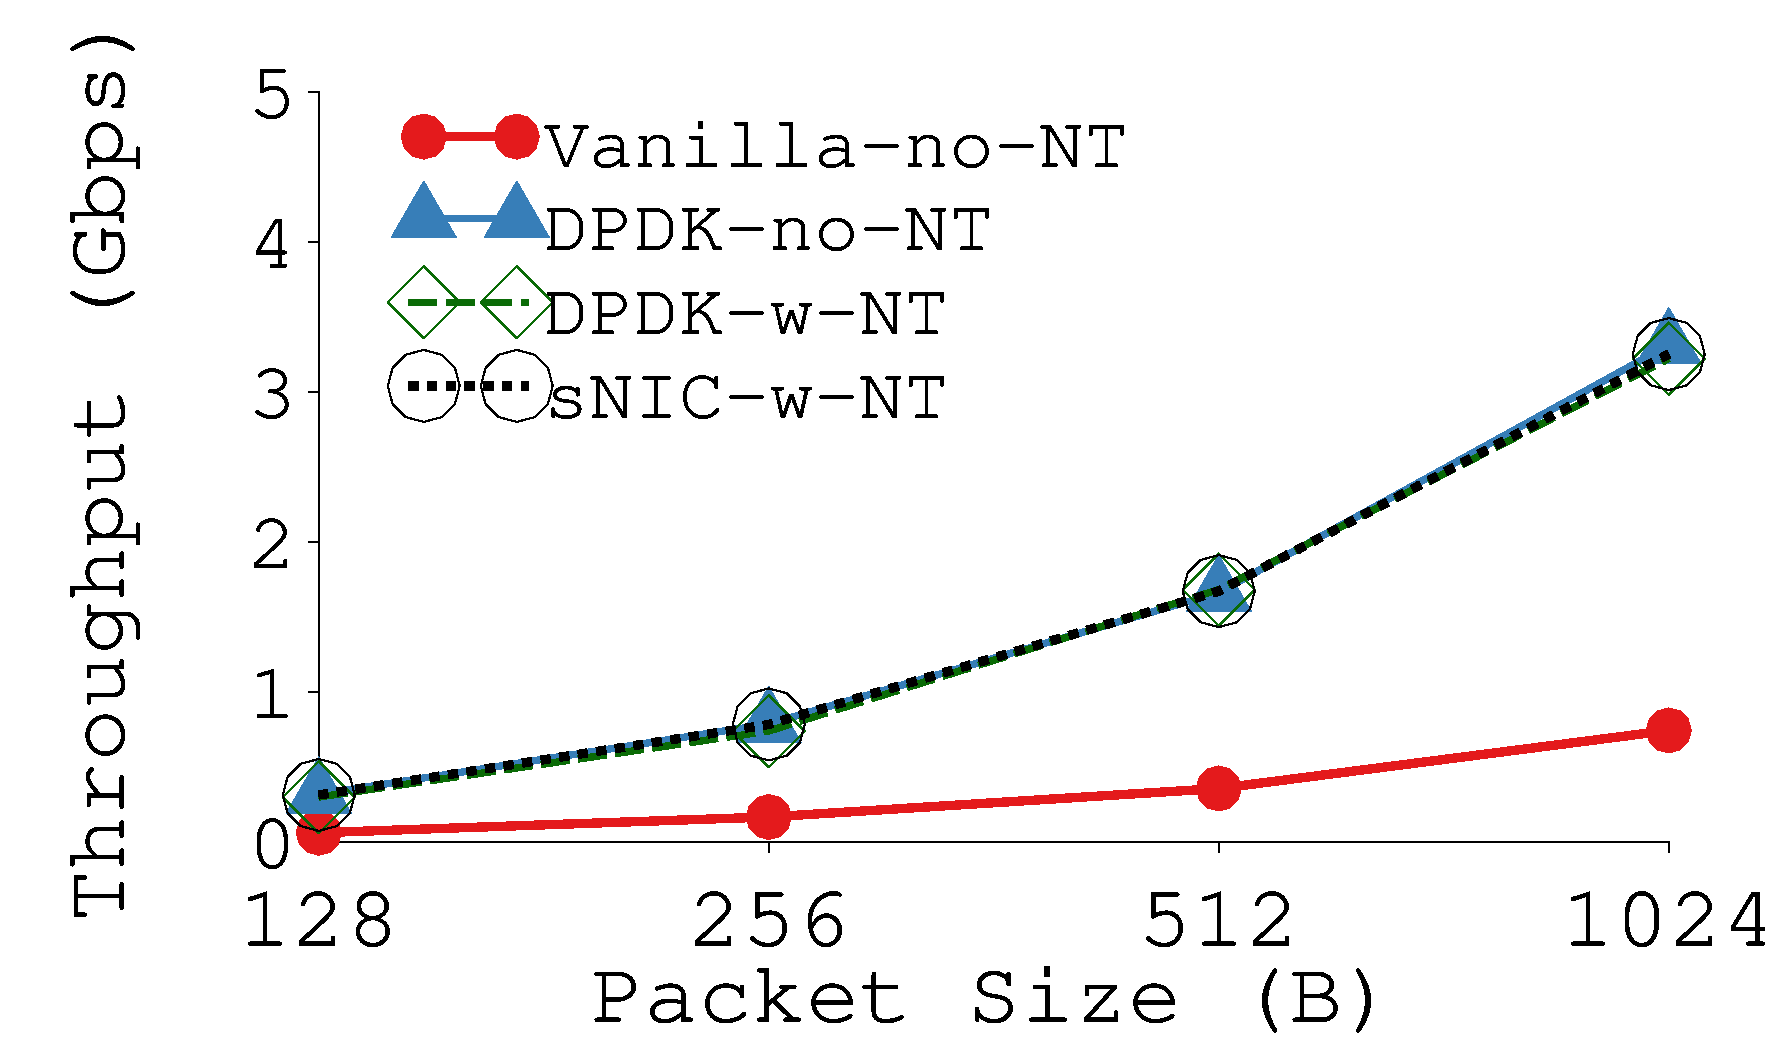
\includegraphics[width=0.5\textwidth]{snic/Figures/g_plot_ovs.pdf}}
\mycaption{fig-ovs}{VPC Performance.}
{
}
\end{center}
\end{figure*}
}

{
\begin{figure}[th]
\begin{center}
\centerline{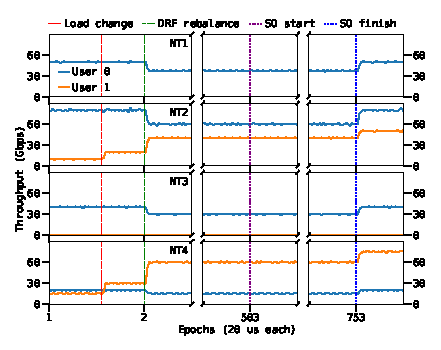
\includegraphics[width=\textwidth]{snic/Figures/drf.pdf}}
\mycaption{fig-drf}{\nt{} Scheduling.}
{
SO: Scaling Out.
}
\end{center}
\end{figure}
}

\bolditpara{\nt-level parallelism.}~~
We then evaluate the effect of \snic's \nt-level parallelism by increasing the number of \nt{}s that could run in parallel.
We compare with PANIC (on our platform), which does not support \nt-level parallelism.
We also show a case where we split \nt{}s into two groups and run these groups as two parallel \nt-chains (half-parallel).
Figure~\ref{fig-nt-parallel} shows the total latency of these schemes.
As expected, running all \nt{}s in parallel achieves the best performance.
The tradeoff is more \nt\ region consumption.
Half-parallel only uses two regions and still outperforms the baseline. % no parallelism PANIC scheme.

\bolditpara{DRF Fairness.}~~
To evaluate the effectiveness of our scheduling policy, we ran the synthetic workloads as described in Figure~\ref{fig-nt-example} and use the default \texttt{EPOCH\_LEN} of 20\mus\ and \texttt{MONITOR\_PERIOD} of 10\ms.
%Here, we set \texttt{EPOCH\_LEN} to 20\mus\ and \texttt{MONITOR\_PERIOD} to 10 epochs or 200us.
Figure~\ref{fig-drf} shows the resulting throughput timeline for different \nt{}s of the two users.
In between epoch 1 and 2, the loads of user2 increased to the second step.
At the next epoch, we run DRF and adjust the allocation. After the DRF algorithm finishes (in around 3\mus), user2 gets a higher (and fairer) allocation of \nt{}2 and \nt{}4, while user1's allocation decreases.
After observing \nt{}2 being overloaded for 10\ms, the \snic\ scales out \nt{}2 by adding one more instance of it at time epoch-503.
After PR is done (in 5\ms), both user1 and user2's throughput increase.



\subsection{End-to-End Application Performance}

We now present our end-to-end application performance conducted on our rack testbed. Because of space constraint, \textit{we move the consolidation experiments of these applications to the Appendix}.

\subsubsection{Disaggregated Key-Value Store}

In this set of experiments, we use one client server and two Clio devices. The Clio devices connect to one \snic\ which connects to the ToR switch. We run YCSB's workloads A (50\% set, 50\% get), B (5\% set, 95\% get), and C (100\% get)~\cite{ycsb-socc10} for these experiments. We use 100K key-value entries and run 100K operations per test, with YCSB's default key-value size of 1\KB\ and Zipf accesses ($\theta=0.99$). 
%The accesses to keys follow the Zipf distribution ($\theta=0.99$).

\bolditpara{Non-replicated YCSB performance and caching.}~~
%Our disaggregated key-value store experiments build on top of the Clio disaggregated memory platform~\cite{clio-arxiv}, where the client side is a regular server and the memory side is two Clio boards.
%Our baseline is the original Clio, which runs a Go-back-N transport on the Clio boards.
%With \snic, we first move the Go-back-N transport as an \nt\ to the \snic\ which connects the two Clio boards to the ToR switch.
%We then add a caching \nt\ to the \snic.
We first evaluate the performance of running YCSB without replication using one client server and one Clio memory device.
Figure~\ref{fig-snic-ycsb} and \ref{fig-snic-ycsb-tput} plot the average end-to-end latency and throughput of running the YCSB workloads with (1) the original Clio, (2) Clio's Go-Back-N transport offloaded to \snic\ (Clio-sNIC), (3) adding caching on top of Clio-sNIC (Clio-sNIC-\$), (4) Clover~\cite{ATC20-pDPM}, a {\em passive} disaggregated memory system where all processing happens at the client side and a global metadata server, (5) HERD~\cite{Kalia14-RDMAKV}, a two-sided RDMA system where both the client and memory sides are regular servers, and (6) HERD running on the NVidia BlueField SmartNIC~\cite{bluefield} (HERD-BF).
\snic's performance is on par with Clio, Clover, and HERD, as it only adds a small overhead to the baseline Clio.
With caching \nt, \snic\ achieves the best performance among all systems, esp. on throughput. 
This is because all links in our testbed are 100\Gbps\ except for the link to the 10\Gbps\ Clio boards. When there is a cache hit at the \snic, we avoid going to the 10\Gbps\ Clio boards.
HERD-BF performs the worst because of the slow link between its NIC and the ARM processor.

\bolditpara{Replicated YCSB performance.}~~
%As many key-value store users desire strong reliability, replication at the memory nodes is usually required.
We then test Clio, Clover, and Clio with \snic\ with replicated write to two Clio devices. HERD does not support replication, and we do not include it here.
Clover performs replicated write in a similar way as the baseline Clio, but with a more complex protocol.
Figure~\ref{fig-ycsb-replication} plots the average end-to-end latency with and without replicated writes using the YCSB A and B workloads.
With \snic's replication \nt, the overhead that replication adds is negligible,
while both Clio and Clover incur significant overheads when performing replication.

\subsubsection{Virtual Private Cloud}
We use one sender server and one receiver server, both running Open vSwitch (OVS)~\cite{ovs-nsdi15}, to evaluate VPC.
Our baseline is the default Open vSwitch that runs firewall, NAT, and AES.
We further improve the baseline by running DPDK to bypass the kernel.
In the \snic\ setup, we connect the sender to an \snic\ and the receiver to another \snic.
Each \snic\ runs the three NFs as a chain.
Figure~\ref{fig-ovs} shows the throughput results.
Overall, we find OVS to be a major performance bottleneck in all the settings. Using DPDK improves OVS performance to some extent.
Compare to running \nt{}s at servers, offloading them to the \snic\ improves throughput, but is still bounded by the OVS running at the endhosts.